
Wir schr"anken nun die Menge der Systeme ein, die wir betrachten wollen, indem wir fordern, dass das System $\mathcal{T}$ gleichzeitig linear und zeitinvariant ist.
Das hei"st, es gilt einerseits, dass ein Eingang $x[\cdot]$ zum System $\mathcal{T}$ mit Ausgang $y[\cdot]$ bei Verz"ogerung zu $x[\cdot - k]$ den entsprechend verz"ogerten Ausgang $y[\cdot - k]$ zur Folge hat.
Gleichzeitig kann der Ausgang des Systems $\mathcal{T}$ f"ur Eingange, die lineare Superpositionen sind als lineare Superposition von den entsprechenden Ausg"angen ausgedr"uckt werden, siehe \Cref{img:disc_sys:linear_sys}.

\subsubsection{Faltungsformel}

Wir wollen die Struktur von \gls{lti}-Systemen ausnutzen, um eine allgemeine und einfache Formel f"ur das Eingangs-Ausgangsverhalten von jenen angeben zu k"onnen.
Als Erstes verallgemeinern wir hierzu \Cref{img:disc_sys:linear_sys} zu beliebigen, aber endlichen Summen, also gegeben ist ein Eingang $x[\cdot]$ der Form
\begin{equation}\label{eq:lti_sys:input}
    x[n] = \Sum{k=1}{K}{a_k \cdot x_k[n]},
\end{equation}

wobei wir wissen, wie die Ausg"ange von jedem $x_k[\cdot]$ zu berechnen sind, also
\[
    y_k[n] = (\mathcal{T}x_k[\cdot])[n].
\]
Dann wissen wir wegen der Linearit"at und \eqref{eq:lti_sys:input}, dass
\begin{equation}\label{eq:lti_sys:superpos}
    y[n] 
        = \left[\mathcal{T}\left(
            \Sum{k=1}{K}{a_k \cdot x_k[\cdot]}
        \right)\right][n] 
        = \Sum{k=1}{K}{
            a_k (\mathcal{T}x_k[\cdot])[n]
        }
        = \Sum{k=1}{K}{
            a_k y_k[n]
        }
\end{equation}
gelten muss.
Es lohnt sich einige Zeit "uber diese Sache zu meditieren und es gibt verschiedene Interpretationen.
\begin{itemize}
    \item Wie bereits erw"ahnt passt dies zur linearen Struktur des Systems $\mathcal{T}$.
    \item Ist ein Eingangssignal aus anderen Signalen zusammengesetzt, dann setzt sich die Reaktion des Systems auf dieses zusammengesetzte Signal aus den Reaktionen auf die Signalbausteine zusammen. 
    Wichtig ist hierbei, dass die Art der Zusammensetzung sich nicht "andert. Die $a_k$ in \eqref{eq:lti_sys:superpos} sind die gleichen, wie in \eqref{eq:lti_sys:input}.
\end{itemize}

Wir wollen nun einen Schritt weiter gehen und eine Menge von $x_k[\cdot]$ angeben, die es erlauben \emph{alle} m"oglichen Signale darzustellen.
Dazu betrachten wir, was geschieht, wenn wir den Einheitssto"s $\delta[\cdot]$ mit einem beliebigen Signal multiplizieren.
Wir rechnen demzufolge f"ur ein beliebiges Signal
\[
x[n] \cdot \delta[n] = \begin{cases}
    x[0] \Text{f"ur} n = 0 \\
    0 \Text{sonst.}
\end{cases}
\]
Wenn wir nun die Einheitsst"o"se verschieben um $k \in \Z$ erhalten wir
\[
    x[n] \cdot \delta[n-k] = \begin{cases}
        x[k] \Text{f"ur} n = k \\
        0 \Text{sonst.}
    \end{cases}
\]
Im Grunde \q{pickt} $\delta[\cdot-k]$ bei Multiplikation den Wert von $x[\cdot]$ an der Stelle $k$ heraus.
Deshalb k"onnen wir nun schreiben
\begin{equation}
    x[n] = \Sum{k \in \Z}{}{
        x[k] \cdot \delta[n-k],
    }
\end{equation}
was nach Definition von $x_k[\cdot] = \delta[\cdot - k]$ genau die Form von \eqref{eq:lti_sys:input} mit $a_k = x[k]$ annimmt.
Die Kernbeobachtung ist nun, dass jedes $x_k[\cdot]$ eine verschobene Kopie von $\delta[\cdot]$ ist. 
Das hei"st, dass wir nun die \gls{lti}-Eigenschaft ausnutzen k"onnen, weil \eqref{eq:lti_sys:superpos} impliziert, dass wir nur $(\mathcal{T}\delta[\cdot])[\cdot]$ berechnen m"ussen und $(\mathcal{T}\delta[\cdot - k])[\cdot]$ sich als $(\mathcal{T}\delta[\cdot])[\cdot - k]$ ergibt.

Wir geben dem Kind nun einen Namen, also definieren wir $h: \Z \rightarrow \C$ als die Antwort des Systems $\mathcal{T}$ auf den Eingang $\delta[\cdot]$, also
\begin{equation}\label{eq:lti_sys:ir}
    h[n] = (\mathcal{T} \delta[\cdot])[n].
\end{equation}
Man nennt $h[\cdot]$ die \emph{Impulsantwort} des Systems.
Dann k"onnen wir also mit \eqref{eq:lti_sys:superpos} folgern, dass
\begin{equation}\label{eq:lti_sys:conv}
    y[n] 
        = (\mathcal{T} x[\cdot])[n] 
        = \Sum{k \in \Z}{}{
            x[k] h[n-k]
        }
\end{equation}
gelten muss.

Das hei"st, dass sich die Antwort $y[\cdot]$ eines diskreten \gls{lti}-Systems aus der \emph{Faltung} des Einganges $x[\cdot]$ mit der Impulsantwort $h[\cdot]$ ergibt.
Wir schreiben in Kurzform
\[
y[n] = (x \ast h)[n] = (h \ast x)[n].
\]
Es wird sich zeigen, dass sich viele Eigenschaften des Systems $\mathcal{T}$ an oft einfacher zu pr"ufenden Eigenschaften der Impulsantwort $h[\cdot]$ ergeben.
Das hei"st, dass $h[\cdot]$ in gewisser Weise das System $\mathcal{T}$ repr"asentiert.
%
\begin{listing}
    \noindent
    \begin{minipage}{0.49\textwidth}
        \strut\vspace*{-\baselineskip}\newline
        \inputminted[firstline=10,lastline=22]{python3}{code/moving_average.py}
    \end{minipage}%
    \begin{minipage}{0.49\textwidth}
        \strut\vspace*{-\baselineskip}\newline
        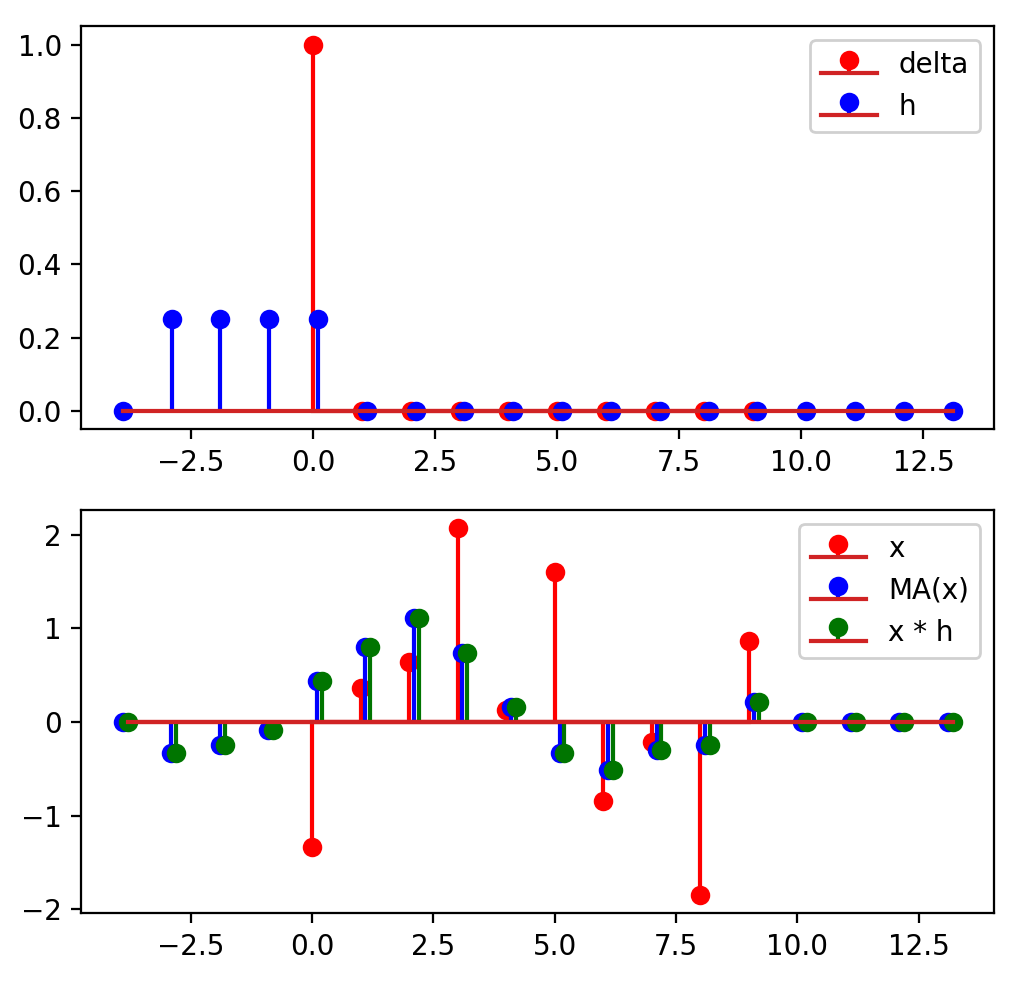
\includegraphics[width=\textwidth]{code/moving_average.png}
    \end{minipage}
    \codecaption{code/moving_average.py}{Gleitendes Mittel mit L"ange $\ell=4$. Wir vergleichen die direkte Berechnung mit der Berechnung "uber die Faltung}\label{py:moving_average}
\end{listing}

In \Cref{py:moving_average} zeigen wir das Verhalten eines gleitenden Mittelwertes (\emph{moving average}), welches sich durch
\[
y[n] = \frac{1}{\ell} \Sum{k=0}{k=\ell}{x[n-k]}
\]
ergibt.
Man sieht sch"on, dass durch das Mitteln die (in diesem Fall) zuf"allige Eingabe-Sequenz am Ausgang gegl"attet erscheint.
Wichtig bei diesem Beispiel ist die Tatsache, dass wir direkt einsehen, dass Anwenung der direkten Formel f"ur das gleitende Mittel aus eine Eingabe $x[\cdot]$ denselben Effekt hat, wie die Faltung mit $h[\cdot]$, das sich aus der Anwendung der Mittelung auf $\delta[\cdot]$ ergibt.

Es lohnt sich, sich einige Eigenschaften der Faltung zu merken. 
Diese sind:
\begin{itemize}
    \item Bi-Linearit"at: Es gilt $(a_1 x_1[\cdot] + a_2 x_2[\cdot]) \ast h[\cdot] = a_1 (x_1 \ast h)[\cdot] + a_2 (x_2 \ast h)[\cdot]$. 
    Dies ist die \q{normale} Linearit"at in den Eing"angen, die sich aus der Linearit"at des Systems $\mathcal{T}$ ergibt. 
    Es gilt aber auch $(x \ast (a_1 h_1 + a_2 h_2))[\cdot] = a_1 (x \ast h_1)[\cdot] + a_2 (x \ast h_2)[\cdot]$.
    Das hei"st, wenn wir ein System $\mathcal{T} = a_1 \mathcal{T}_1 + a_2 \mathcal{T}_2$ gegeben haben, dann ist die Impulsantwort des Systems $\mathcal{T}$ die gleiche Linearkombination der Impulsantworten $h_1[\cdot]$ und $h_2[\cdot]$ der beiden Systeme $\mathcal{T}_{1,2}$.
    Das hei"st wiederum, dass \gls{lti}-Systeme selbst ein linearer Raum sind!
    Wir sprechen hier von \emph{Bi}-Linearit"at, weil die Faltung eben linear in zwei Argumenten ist.
    \item Die Faltung ist assoziativ: Es gilt also, dass $(x \ast h_1) \ast h_2 = x \ast (h_1 \ast h_2)$. 
    Dies impliziert, dass die Verkettung von zwei \gls{lti}-Systemen wieder ein \gls{lti}-system ergibt, wobei sich die Impulsantwort der Verkettung durch Faltung der beiden Impulsantworten der verketteten Systeme ergibt.
    \item Kommmutativit"at: Es gilt $h_1 \ast h_2 = h_2 \ast h_1$, demnach auch, dass $x \ast (h_1 \ast h_2) = x \ast (h_2 \ast h_1)$.
    Das hei"st erstaunlicherweise, dass man verkettete \gls{lti}-Systeme in ihrer Reihenfolge vertauschen kann, ohne das Eingangs-Ausgangsverhalten des Gesamtsystems zu beeinflussen.
\end{itemize}

\begin{listing}
    \noindent
    \begin{minipage}{0.40\textwidth}
        \strut\vspace*{-\baselineskip}\newline
        \inputminted[firstline=10,lastline=33]{python3}{code/ramp_ma.py}
    \end{minipage}%
    \begin{minipage}{0.59\textwidth}
        \strut\vspace*{-\baselineskip}\newline
        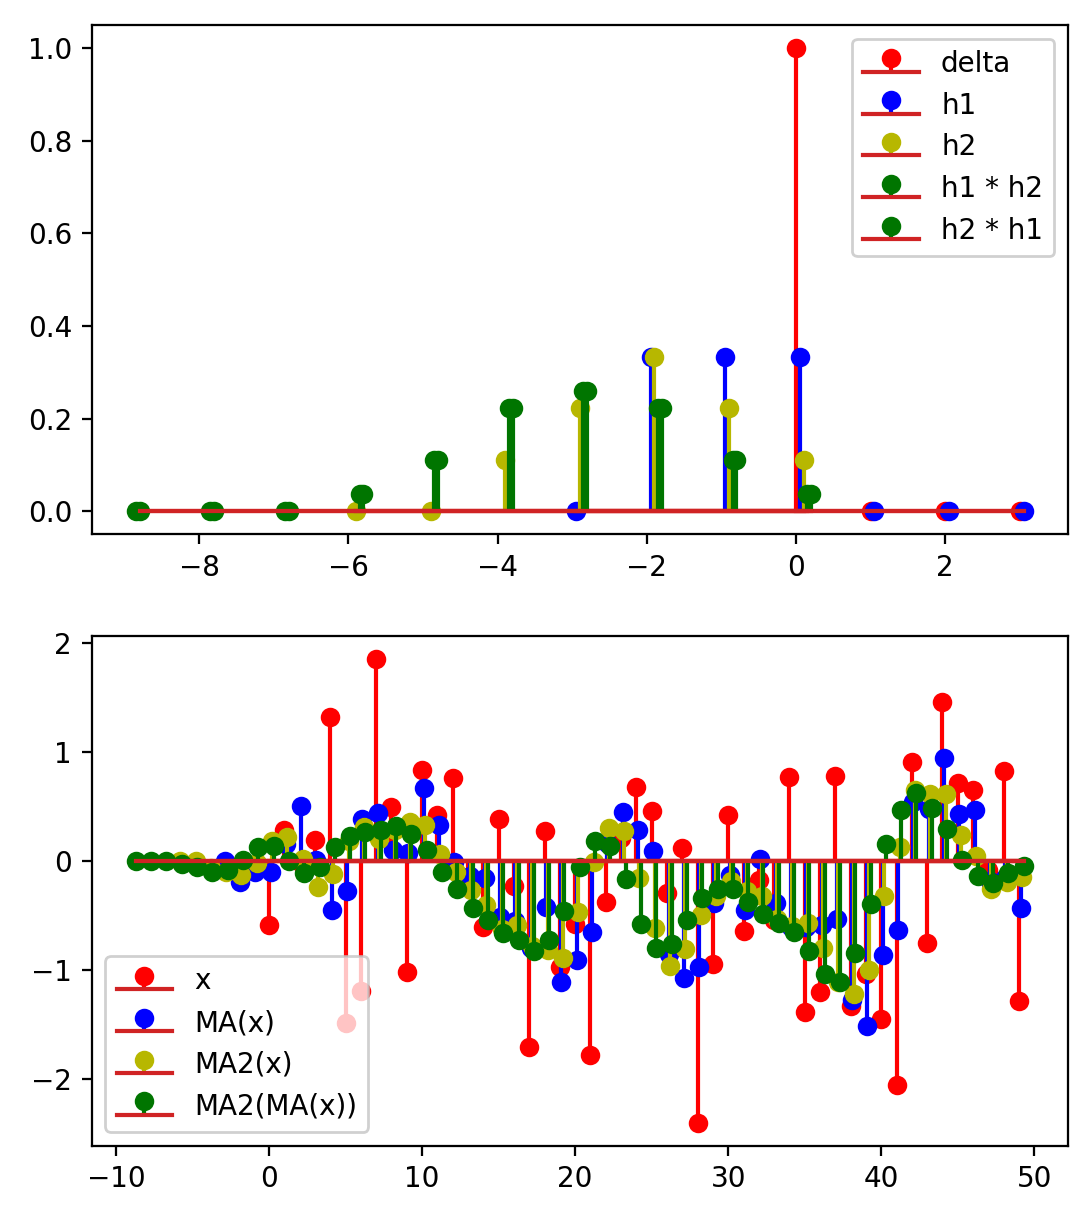
\includegraphics[width=\textwidth]{code/ramp_ma.png}
    \end{minipage}
    \codecaption{code/ramp_ma.py}{Verkettung von mehreren Moving Averages der L"ange $\ell = 3$.}\label{py:ramp_ma}
\end{listing}
%
In \Cref{py:ramp_ma} untersuchen wir einige der oben genannten Eigenschaften.
Einerseits sehen wir, dass die Impulsantwort von $\texttt{MA}(\texttt{MA2}(\cdot))$ mit der von $\texttt{MA2}(\texttt{MA}(\cdot))$ identisch ist. Wir haben also Kommutativit"at nachgepr"uft.
Wir sehen au"serdem, dass sich die Impulsantwort der Verkettung aus Faltung der einzelnen Impulsantworten ergibt.
Aus dem abgetasteten \q{Rechteck} wird nach nochmaliger Anwendung ein abgetastetes, aber breiteres, \q{Dreieck}, was schlussendlich zu einer abgetasteten, st"uckweise quadratischen, Impulsantwort wird.
Generell kann man das komplette System als eine dreifache Verkettung gleitender Mittel der L"ange $\ell=3$ verstehen.
Au"serdem best"atigt \Cref{py:ramp_ma} bei Vergleich der verschiedenen Ausg"ange, dass wiederholtes Mitteln am Ausgang mit Anzahl der Mittelungen zunehmend \q{glattere} Signale erzeugt.
%
\subsubsection{Eigenschaften von \texorpdfstring{\acrshort{lti}}{LTI}-Systemen}
%
\begin{itemize}
    \item stabilitaet: $h[n]$ muss absolut summierbar sein, gegen $0$ gehen
    \item beispiel 2.3.6. (fuer uebung irgendwas ausdenken)
    \item \gls{fir} vs. \gls{iir}
\end{itemize}

\subsection{Kreuz- und Autokorrelation}\label{corr}

\begin{itemize}
    \item Definition
    \item eigenschaften
    \item synthetisches beispiel schwingung + noise, akf zeigt periodizitaet
    \item beispiel mit woelfer sunspot numbers
    \item beispiel mit m-sequenzen, niklas einladen, schaltung zeigen
    \item monster uebung: 2.65
\end{itemize}